\section{Metodología}

\subsection{Identificación de la Situación actual}

% Pocas entidades que brinden todos estos servicios.

Actualmente en la región de Valparaíso existen diversos servicios enfocados a
bandas de música, pero ninguno de ellos ofrece el servicio completo consistente en salas de
grabación, salas de ensayo, promoción/difusión, traslado a eventos, etc.

Además, la región se caracteriza por su alta oferta de actividades recreativas,
enfocándose en gran parte al área turística y recreacional a lo largo de todo el año.

Dentro de éste contexto, existen a su vez un sinnúmero de bares y pubes en los que
múltiples bandas ofrecen sus servicios gratuitamente en búsqueda de promoción
propia, para lograr ser más conocidas y aumentar sus posibilidades de trabajo.

Si las bandas no tuvieran que
gastar tanto esfuerzo en la promoción y búsqueda de eventos en los que estar
presentes, podrían dedicar más tiempo a la creación musical, y generando
alianzas estratégicas con los diferentes locales de recreación se puede generar
una mayor difusión de las bandas que presenten en cada uno de ellos.

\subsection{Situación Base}

% Corresponde a la situación actual optimizada.
% ¿Qué pasa si no se realiza el proyecto?
% La optimización de la situación actual es a nivel de gestión y de eficiencia,
%  implica la realización de inversiones significativas.

El proyecto se iniciará desde cero,
y por el momento no existen alternativas que sean equivalentes al servicio completo
que se ofrecerá.

Las únicas aproximaciones podrían ser los centros que hoy en día
tienen a lo más sala de ensayo y grabación, pero no son comparables
debido a que aquellas características sólo son una parte de la idea propuesta.

\subsection{Situación con proyecto}

% Se proyecta como sería el escenario realizando el proyecto.
% Se analizan todos los impactos, positivos o negativos, que generará la realización
%  del proyecto.

Tomando en cuenta la situación actual para todos los grupos musicales
que nacen en Chile se estaría provocando un cambio radical en la mentalidad
de las bandas emergentes, pues se estaría creando un proyecto
nunca antes visto, el cual fomentaría la experiencia musical en Chile.

Al ofrecer un conjunto de servicios relacionados y con el mismo objetivo,
lograr que una banda se posicione como una banda famosa a nivel nacional,
es difícil que cualquier banda emergente rechace la oferta.

Pero, además de fomentar la madurez musical de las nuevas bandas
de Chile, se está potenciando la música en chile,
lo que puede provocar a largo plazo un cambio de mentalidad
en la población chilena, para poder considerar aún más
lo que vendría siendo el producto nacional.

\subsection{Comparación situación base y situación con proyecto}

Actualmente no existe oferta alguna del servicio propuesto, por lo que el
público objetivo debe encargarse de gran parte de la difusión y promoción.

\subsection{Separabilidad de Proyectos}

% Las unidades estratégicas son aquellas que no se pueden separar.
% Dividir el proyecto en dos o más subproyectos.
% Los proyectos son separables en la medida que se pueda identificar un producto
%  o servicio a transferir y un precio de transferencia.
%
% Explicar que para simplificar el proyecto no se planeará dividir el proyecto
%  en diferentes empresas o cosas por el estilo.
% Nuestro proyecto puede llevarse a cabo a través de una sola empresa que preste
%  todos los servicios anteriormente mencionados, esto porque justamente uno los
%  objetivos es ofrecer el servicio completo a nuestros clientes, evitando que
%  deban recurrir a diferentes instancias y abaratando costos (Juan).

Debido a las características del presente proyecto
se puede fácilmente notar que es perfectamente separable
en varias unidades estratégicas, como:

\begin{itemize}
	\item Salas de ensayo.
	\item Estudios de grabación.
	\item Posicionamiento en redes sociales y web 2.0.
	\item Salas de eventos.
\end{itemize}

Si bien es cierto,
cada uno de los puntos anteriormente señalados puede
verse como un producto final que será adquirido
por los potenciales clientes a un determinado
valor, no va de la mano con nuestra propuesta.

A lo largo de Chile existen distintas
empresas que brindan algunos de estos servicios,
pero ninguna ha realizado la labor de poder
ofrecer un producto más generalizado y completo,
es por eso que no se planea dividir el proyecto,
pues se estaría poniendo a disposición de terceros
alguno de los servicios que serían los pilares fundamentales
de nuestra propuesta, ya que se pretende provocar
la confianza de los clientes, al poder recurrir
a nosotros y brindarles un servicio completo
de primera calidad, evitando tener que buscar
en diferentes lugares, a veces en distintas regiones
de Chile, intentando conseguir  una cierta
cantidad concreta de elementos vitales
para lo que es la evolución de una \emph{``Banda Musical''}.

\subsection{Métodos de medición de beneficios y costos }

% Obedece a procedimientos establecidos de valoración.
% Definición de la forma de evaluación de los movimientos de fondos.
%  (permiten construir un flujo de caja)
% Identificación de los costos de inversión, operaciones,
%  beneficios directos e indirectos.
%
% El procedimiento general consiste en la identificación de las variables,
%  ya sean de beneficios y costos; luego la cuantificación de ellas en unidades
%  física, siempre y cuando las variables sean factibles de cuantificar; y 
%  posteriormente se procede a la valoración monetaria, es decir, asignarle
%  un precio o costo a ellas.

\subsubsection{Inversión}
\begin{itemize}
	\item Arriendo de local:
			Se necesita un local ubicado en lo ideal en el sector céntrico de Viña del Mar,
			con suficiente espacio para dos salas de ensayo, una sala de grabación, una oficina
			y un salón de eventos.
			Cada sala de ensayo debe ser de al menos 12 metros cuadrados,
			la sala de grabación y la oficina de al menos 9 metros cuadrados cada una,
			el salón de eventos podría estar ubicado perfectamente en otro lugar,
			o en el mismo establecimiento, para favorecer la llegada de público.
	\item Equipos:
			Se necesitarán amplificadores, altavoces, mesas, reproductores, entre otros.
	\item Instrumentos:
			Se necesitarán diversos instrumentos entre los cuales destacan guitarras, bajos, baterías,
			teclados, micrófonos, entre otros.
	\item Publicidad:
			Este punto será el más importante, pues se necesita llegar a todos los rincones posibles,
			por lo que la inversión en publicidad es esencial.
			Se requerirán anuncios publicitarios en radios, internet, afiches en centros de eventos,
			pubes, etc, teniendo como principal misión, comunicar el proyecto en lugares
			frecuentados por músicos.
\end{itemize}

\subsubsection{Ingresos}
\begin{itemize}
	\item Arriendo Sala Ensayo:
			Se obtendrán ingresos por el concepto de arriendo por hora de la sala de ensayos.
	\item Contratación grabación disco:
			Se prestará el servicio de grabación y asesoría técnica para la grabación de un
			disco con los temas seleccionados por la banda.
			El valor dependerá de la duración del disco y de la complejidad del equipo
			e instrumentos necesarios para su grabación.
	\item Contratación posicionamiento web:
			Se prestarán servicios de publicidad para bandas que deseen difusión a través
			de internet, haciendo uso de redes sociales y en caso de que la banda no posea
			sitio web, también puede pagar por la creación y mantención de uno.
	\item Traslados:
			Se ofrecerá el servicio de traslado de bandas a distintos eventos en la zona.
	\item Contratación sistema completo:
			Se ofrecerán todos los servicios anteriores por un precio mucho más conveniente
			para los clientes, sin duda una de las características diferenciadoras de
			nuestra empresa con respecto a lo que se ofrece en el mercado.
\end{itemize}

\subsubsection{Costos fijos}
\begin{itemize}
	\item Salarios:
			Costo fijo mensual para pago de empleados de la empresa entres los cuales se cuentan:
			técnicos en sonido, secretaria y ayudantes.
	\item Servicios básicos:
			Costo de agua,luz y otros inherentes a la mantención del local.
	\item Servicios adicionales:
			Costo de servicios adicionales como teléfono e internet.
	\item Seguros:
			Seguros de robo e incendio.
	\item Mantención:
			Costo fijo mensual de mantención de aseo, reparación de equipos, entre otros.
\end{itemize}


\subsection{Método de evaluación de rentabilidad que se usará}

Es posible encontrar variados
métodos para valorizar las inversiones, 
los cuales se pueden agrupar en dos grandes categorías: los métodos \emph{dinámicos} y los métodos \emph{estáticos}.

Los \emph{métodos estáticos} no consideran
el tiempo como un factor importante,
es decir, que no se considerará el momento en el cual
pueda existir una salida o entrada de dinero al
proyecto.

Algunos ejemplos de \emph{métodos estáticos} son:
\begin{itemize}
	\item El método del Pay-Back o Plazo de recuperación.
	\item El método del flujo neto de caja (Cash-Flow estático).
	\item El método de la Tasa de rendimiento contable.
\end{itemize}

Por otro lado,
los \emph{métodos dinámicos}, van a suplir el problema
que poseen los métodos estáticos, ya que si van a tomar
en consideración el tiempo en que se producen entradas
o salidas de dinero.

Algunos ejemplos de \emph{métodos dinámicos} son:
\begin{itemize}
	\item La Tasa de Rentabilidad Interna (T.I.R).
	\item La Tasa de Rentabilidad Interna Modificada(T.I.R.M).
	\item El Valor Actual Neto (V.A.N).
	\item El Pay-Back dinámico (o descontado).
\end{itemize}

El problema que se podría considerar es que éstos métodos
nos entregan información de una cierta porción del
proyecto, por lo cual es muy recomendado poder utilizar
el complemento de éstos tres métodos, para poder
tener una visión mucho más completa de la situación
actual del proyecto.

Es por la razón anterior, que el proyecto utilizará
los métodos dinámicos nombrados anteriormente.

\subsubsection{Tasa Interna de Rentabilidad}

Cuando se habla de Tasa Interna de Rentabilidad (T.I.R.)
se refiere a una tasa de descuento que produce que el Valor Actual Neto (V.A.N),
de una inversión igual a cero.

Pero, ¿De qué nos sirve éste método?

Si la T.I.R. que resulte va a superior o igual a la tasa exigida por el inversor,
tomando en consideración variadas alternativas, la que nos entregue
una T.I.R. mayor, será más conveniente.

Pero, ¿Qué tan complejo es su cálculo?

Éste método es conocido por ser muy difícil de calcular (método iterativo),
pero hay variadas alternativas que nos ayudarán a tener un trabajo más fácil, ya sean utilizando
planillas de cálculo, técnicas matemáticas como la interpolación lineal, o calculadoras
especializadas.

%	Pero la más importante crítica del método (y principal defecto) es la inconsistencia
%	matemática de la T.I.R. cuando en un proyecto de inversión hay que efectuar otros
%	desembolsos, además de la inversión inicial, durante la vida útil del mismo, ya sea debido a
%	pérdidas del proyecto, o a nuevas inversiones adicionales.
%	La T.I.R. es un indicador de rentabilidad relativa del proyecto, por lo cual cuando se hace
%	una comparación de tasas de rentabilidad interna de dos proyectos no tiene en cuenta la
%	posible diferencia en las dimensiones de los mismos. Una gran inversión con una T.I.R.
%	baja puede tener un V.A.N. superior a un proyecto con una inversión pequeña con una
%	T.I.R. elevada.

\subsubsection{Tasa Interna de Rentabilidad Modificada}
	Esta tasa fue diseñada con la finalidad de superar las deficiencias de la T.I.R. 
	La tasa T.I.R.M tiene en consideración la posibilidad de reinvertir los flujos incrementales de fondos del proyecto a una tasa equivalente al costo de capital de la empresa, a diferencia de la T.I.R que supone la reinversión de los flujos a la tasa interna de retorno del proyecto.
	Esta tasa también se conoce como tasa de retorno o recuperación externa.

\subsubsection{Valor Actual Neto}

Se entiende como Valor Actual Neto (V.A.N) de una determinada inversión realizada,
como la sumatoria de todos los valores actualizados, considerando todos los flujos
de caja esperados (netos), los cuales se pueden deducir del valor inicial
que se utilizó cuando se comenzó la inversión, lo cual claramente es una ventaja.

Las características fundamentales para que un proyecto sea rentable son:
\begin{itemize}
	\item Se considera un proyecto $A$ y un proyecto $B$, se calcula los V.A.N.
		  de cada uno, $vanA$ y $vanB$, el que posea un V.A.N. más alto
		  será el proyecto más rentable.
	\item Si el V.A.N. posee un valor positivo, es rentable, en cambio
		  si su valor es nulo, se sabrá que la rentabilidad será equivalente
		  a disponer los fondos en un mercado determinado, considerando un cierto
		  interés equivalente a la tasa de descuento que se ha utilizado.
\end{itemize}

Debido a que el presente proyecto será financiado en su totalidad mediante un préstamo,
se fijará el valor de la tasa de interés, se utilizará el costo de la deuda.


%	Conocido bajo distintos nombres, es uno de los métodos más aceptados (por no decir el que
%	más).
%	Por Valor Actual Neto de una inversión se entiende la suma de los valores actualizados de
%	todos los flujos netos de caja esperados del proyecto, deducido el valor de la inversión
%	inicial.
%	Si un proyecto de inversión tiene un VAN positivo, el proyecto es rentable. Entre dos o más
%	proyectos, el más rentable es el que tenga un VAN más alto. Un VAN nulo significa que la
%	rentabilidad del proyecto es la misma que colocar los fondos en él invertidos en el mercado
%	con un interés equivalente a la tasa de descuento utilizada. La única dificultad para hallar el
%	VAN consiste en fijar el valor para la tasa de interés, existiendo diferentes alternativas.
%	
%	Como ejemplo de tasas de descuento (o de corte), indicamos las siguientes:
%		a) Tasa de descuento ajustada al riesgo es la suma entre Interés que se puede obtener
%		   del dinero en inversiones sin riesgo (deuda pública) y la prima de riesgo.
%		b) Coste medio ponderado del capital empleado en el proyecto.
%		c) Coste de la deuda, si el proyecto se financia en su totalidad mediante préstamo o
%		   capital ajeno.
%		d) Coste medio ponderado del capital empleado por la empresa.
%		e) Coste de oportunidad del dinero, entendiendo como tal el mejor uso alternativo,
%		   incluyendo todas sus posibles utilizaciones.
%	
%	La principal ventaja de este método es que al homogeneizar los flujos netos de Caja a un
%	mismo momento de tiempo (t=0), reduce a una unidad de medida común cantidades de
%	dinero generadas (o aportadas) en momentos de tiempo diferentes. Además, admite
%	introducir en los cálculos flujos de signo positivos y negativos (entradas y salidas) en los
%	diferentes momentos del horizonte temporal de la inversión, sin que por ello se distorsione
%	el significado del resultado final, como puede suceder con la T.I.R.
%	Dado que el V.A.N. depende muy directamente de la tasa de actualización, el punto débil
%	de este método es la tasa utilizada para descontar el dinero (siempre discutible). Sin
%	embargo, a efectos de “homogeneización”, la tasa de interés elegida hará su función
%	indistintamente de cual haya sido el criterio para fijarla.
%	
%	El V.A.N. también puede expresarse como un índice de rentabilidad, llamado Valor neto
%	actual relativo, expresado bajo la siguiente fórmula:
%		VAN relativo = VAN de la inversion / Inversion
%	O bien en forma de tasa (%):
%	
%		Tasa VAN relativo = VAN de la inversion / Inversion * 100
%
\subsubsection{Pay-Back dinámico}

El Pay-Back dinámico busca solucionar el problema principal del Pay-back estático,
el cual es que no considera los valores actuales de los flujos de caja de los últimos
periodos, por lo que un método dinámico siempre será más actualizado, pero incompleto.

El Pay-Back dinámico corresponde al periodo de tiempo necesario para poder recuperar
el capital invertido en cierto proyecto.

La idea principal es poder calcularlo para complementar el estudio de la valorización
del riesgo de una inversión determinada, en casos complejos de predecir la tasa de
depreciación de la inversión, que ocurre muy frecuentemente.

% ------------------------ lo de abajo no iría ---------------------------


% Es costumbre evaluar los proyectos mediante la aplicación de criterios convervadores
%  (VAN y TIR), no obstante en algunos proyectos será necesario emplear criterios específicos
%  como por ejemplo, para el caso de evaluación de proyectos sociales del área salud, un
%  indicador puede ser el número de pacientes senados o atendidos anualmente.
% El contenido de la metodología de evaluación varía en tamaño de 10 a 20 páginas.
%----------------
%
%
%Rentabilidad
%
%Para obtener la rentabilidad financiera del proyecto se utilizara el indicador ROE (return on
%equity), el cual relaciona el beneficio económico con los recursos necesarios para obtener ganancia.
%Luego, para demostrar porque fue ganada una cierta rentabilidad financiera se utilizara la Fórmula de
%Du Pont, la cual analiza detalladamente las causas que generaron la rentabilidad.
%
%ROE = Beneficio Neto / Patrimonio Neto
%
%Formula de Du Pont = Beneficio Neto / ventas × Patrimonio Neto / ventas
%
%Evaluación de la inversión
%	Dentro de los modelos de evaluación de inversiones evaluamos los seis métodos
%	existentes determinando el más acorde a nuestro proyecto:
%Flujo neto de caja
%	Def 1:
%	Este método comprende la suma de todos los cobros menos todos los pagos efectuados durante
%	la vida útil del proyecto de inversión. Debido a su poca utilidad practica de este método consideramos
%	descartarlo.
%
%	Def 2:
%	Por Flujo neto de Caja, se entiende la suma de todos los cobros menos todos los pagos
%	efectuados durante la vida útil del proyecto de inversión. Está considerado como el método
%	más simple de todos, y de poca utilidad práctica.
%	Existe la variante de Flujo neto de Caja por unidad monetaria comprometida, la cual es el
%	cociente entre el Flujo neto de Caja y la Inversión inicial.
%
%PayBack estático
%	Def 1:
%	Debido a que este método considera aquellos proyectos cuyos beneficios permiten recuperar
%	más rápidamente la inversión, consideramos que no es apropiado para nuestro caso por el largo plazo
%	de recuperación de la inversión.
%
%	Def 2:
%	Es el número de años que la empresa tarda en recuperar la inversión. Este método
%	selecciona aquellos proyectos cuyos beneficios permiten recuperar más rápidamente la
%	inversión, es decir, cuanto más corto sea el periodo de recuperación de la inversión mejor
%	será el proyecto.
%	Los inconvenientes que se le atribuyen, son los siguientes:
%	
%		a) El defecto de los métodos estáticos (no tienen en cuenta el valor del dinero en las
%		   distintas fechas o momentos)
%		b) Ignora el hecho de que cualquier proyecto de inversión puede tener corrientes de
%		   beneficios o pérdidas después de superado el periodo de recuperación o reembolso.
%	
%	Puesto que el plazo de recuperación no mide ni refleja todas las dimensiones que son
%	significativas para la toma de decisiones sobre inversiones, tampoco se considera un
%	método completo para poder ser empleado con carácter general para medir el valor de las
%	mismas.
%
%Tasa de rendimiento contable
%	Def 1:
%	Este método se basa en el concepto del Cash-Flow en vez de cobros y pagos, a pesar que nos
%	permite hacer los cálculos rápidamente al no tener que elaborar estados de cobros y pagos, sin embargo
%	no tiene en cuenta la liquidez del proyecto lo cual pudiera comprometer la viabilidad de nuestro pro-
%	yecto, debido a esta causa hemos considerado no tomar en cuenta este método.
%	Por lo tanto podemos decir que ninguno de estos métodos estáticos son convenientes de usar en
%	nuestro proyecto.
%
%	Def 2:
%	Este método se basa en el concepto de Cash-Flow, en vez de cobros y pagos (Cash-Flow
%	económico).
%	
%	La principal ventaja, es que permite hacer cálculos más rápidamente al no tener que
%	elaborar estados de cobros y pagos (método más engorroso) como en los casos anteriores.
%	
%	La definición matemática es la siguiente:
%	
%	[(Beneficios + Amortizaciones)/Años de duración del proyecto] / Inversión inicial del
%	proyecto
%	
%	
%	El principal inconveniente, además del defecto de los métodos estáticos, es que no tiene en
%	cuenta la liquidez del proyecto, aspecto vital, ya que puede comprometer la viabilidad del
%	mismo.
%	Además, la tasa media de rendimiento tiene poco significado real, puesto que el
%	rendimiento económico de una inversión no tiene porque ser lineal en el tiempo.
%
%
%
%El Cash-Flow actualizado
%	Def 1:
%		Podemos considerar este método como una variante de la Tasa de rendimiento contable. Toma
%		los beneficios brutos antes de amortizaciones para cada uno de los años de la vida útil del proyecto, y
%		los actualiza o descuenta conforme a una tasa de interés. Permite unos cálculos más simples que los
%		métodos que trabajan con previsiones de cobros y pagos.
%		
%		Sin embargo, al contrario que la tasa contable, este método si tiene en cuenta la liquidez del
%		proyecto a nivel de cash-flow en cada uno de los años que contempla la inversión.
%		Como podemos analizamos anteriormente, cada uno de estos últimos tres métodos contemplan
%		un aspecto diferente del problema, considerando que no es problema usar estos tres métodos simultá-
%		neamente, por lo tanto utilizaremos estos tres métodos de manera que nos proveerán de una visión más
%		completa de la inversión.
%
%		Def 2:
%		Podemos considerar esté método como una variante de la Tasa de Rendimiento contable.
%		Toma los beneficios brutos antes de amortizaciones para cada uno de los años de la vida
%
%		útil del proyecto, y los actualiza o descuenta conforme a una tasa de interés. Permite unos
%		cálculos más simples que los métodos que trabajan con previsiones de cobros y pagos.
%		Sin embargo, al contrario que la tasa contable, este método si tiene en cuenta la liquidez del
%		proyecto a nivel del cash-flow generado en cada uno de los años del horizonte temporal de
%		la inversión.
%		Por todo lo expuesto anteriormente, utilizaremos el Valor Actual Neto (V.A.N) como
%		método para medir la rentabilidad de nuestra planta de cerveza artesanal, ya que es el
%		método más aceptado, homogéneo y el que menos dificultades presenta.
%

\subsection{Programación de las actividades de la evaluación del proyecto (Carta Gantt)}

\begin{figure}[h]
\centering
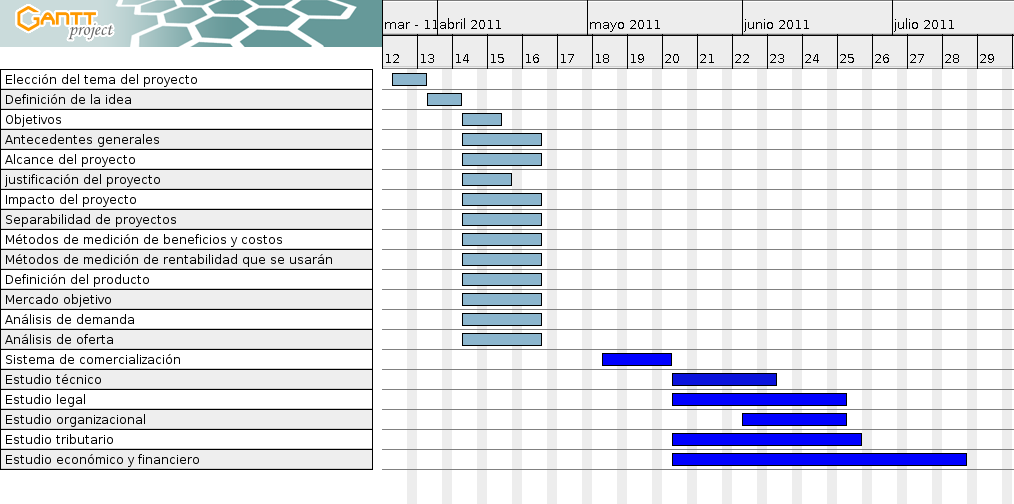
\includegraphics[scale=0.4]{img/carta_gantt.png}
\caption[Carta Gantt de las actividades de la evaluación del proyecto]{Carta Gantt de las actividades de la evaluación del proyecto}
\end{figure}
% Considerar sólo hasta fin de semestre, indicando cuando se realizará los estudios de mercado y esas cosas.
%
% Hay que definir una lista de actividades a realizar,
%

%Estudio Mercado.
%	Definición de producto. 1-2
%	Mercado objetivo. 1-3
%	Analisis de demanda.3-5
%	Analisis de oferta.3-5
%	Sistema de comercialización.4-7
%Estudio Técnico
%	Tamaño del proyecto.8
%	Localización del proyecto.8-9
%	Ingeniería del proyecto.8-13
%	Estimación y analisis de costo.12-13
%Estudio Socetario.8-9
%Estudio Legal.8-10
%Estudio Organizacional.11-13
%Estudio Tributario.8-10
%Estudio Ambiental.12-13
%Estudio Economico y financiero.14-16
%
%---------
%
%Estudio de Mercado 1-2
%Estudio Técnico 3-5
%Estudio organizacional 5-6
%Estudio legal 7-8
%Estudio ambiental 9-10
%Estudio economico 11-12
%Estudio financiero  12-14
